% Emacs, this is -*-latex-*-
\documentclass[convert={density=300,size=1080x800,outext=.png}]{standalone}
\usepackage[utf8]{inputenc}
%\usepackage{hyperref}
\usepackage{siunitx,verbatim}
%\usepackage[english]{babel} 
\usepackage{wrapfig,multimedia}
\usepackage[safe]{tipa}
\usepackage{tikz,framed}
\usepackage{multirow}
\usepackage[T1]{fontenc} 
\usepackage{framed}
\usepackage{tipa}

% pdftoppm -png -r 600 out.pdf > out.png
% convert -density 300 file.pdf -quality 90 file.png

\usetikzlibrary{positioning,calc,shapes.callouts,shapes.arrows}
\usetikzlibrary{mindmap,backgrounds,automata,fit,arrows,decorations.markings}

\sisetup{per-mode=symbol,
range-phrase = { ... },
}



\begin{document}

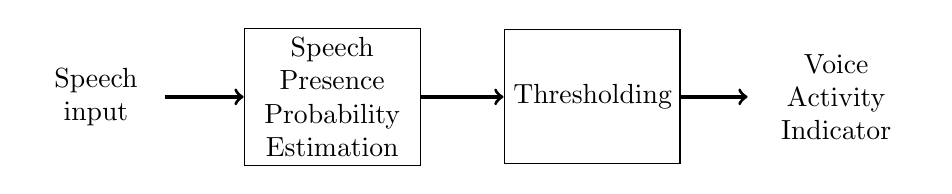
\begin{tikzpicture}

   \node at (0,0) (speech) {\parbox{1.5cm}{\centering Speech input}};  
   \node[draw,minimum height=1.7cm,minimum width=2cm] at (3,0) (spp) {\parbox{2cm}{\centering Speech Presence Probability Estimation}};
   \node[draw,minimum height=1.7cm,minimum width=2cm] at (6.3,0) (thresh) {\parbox{2cm}{\centering Thresholding}};
   \node at (9.4,0) (vad) {\parbox{2cm}{\centering Voice Activity Indicator}};

   \draw[very thick,->] (speech) -> (spp);
   \draw[very thick,->] (spp) -- (thresh);
   \draw[very thick,->] (thresh) -- (vad);
\end{tikzpicture}
  

\end{document}
